\subsection{Slučaj upotrebe: Izmena zaposlenog i korisničkog naloga}

\subsubsection*{Kratak opis:}

Administrator menja podatke o zaposlenom, njegove uloge i prava pristupa, resetuje lozinku ili otključava nalog.

\subsubsection*{Akteri:}
\begin{itemize}
	\item \textbf{Administrator} -- upravlja evidencijom zaposlenih i njihovim nalozima.
\end{itemize}

\subsubsection*{Preduslovi:}
\begin{itemize}
	\item Administrator je prijavljen na sistem.
	\item Zaposleni čiji se podaci menjaju postoji u sistemu.
\end{itemize}

\subsubsection*{Postuslovi:}
\begin{itemize}
	\item Podaci o zaposlenom i njegovom nalogu su ažurirani.
	\item Sistem je evidentirao promenu.
\end{itemize}

\subsubsection*{Osnovni tok:}
\begin{enumerate}
	\item Administrator bira opciju „Upravljanje zaposlenima“.
	\item Sistem prikazuje listu zaposlenih sa pretragom i filtriranjem po imenu, ulozi i statusu naloga.
	\item Administrator bira zaposlenog.
	\item Sistem prikazuje njegove podatke, uloge, prava i status naloga.
	\item Administrator menja željene podatke.
	\begin{itemize}
		\item Ukoliko menja ulogu ili prava pristupa, izvršava se podtok P1.
		\item Ukoliko resetuje lozinku ili otključava nalog, izvršava se podtok P2.
	\end{itemize}
	\item Administrator potvrđuje izmene.
	\item Sistem proverava ispravnost podataka.
	\item Sistem čuva izmene i evidentira ih.
	\item Sistem prikazuje potvrdu i ažuriranu listu.
\end{enumerate}

\subsubsection*{Podtokovi:}

\paragraph*{P1: Promena uloge i prava pristupa}
\begin{enumerate}
	\item Sistem prikazuje dostupne uloge i pojedinačna prava.
	\item Administrator dodaje ili uklanja ulogu, odnosno pojedinačna prava.
	\item Sistem prikazuje rezime izmena i nastavlja se od koraka 6 osnovnog toka.
\end{enumerate}

\paragraph*{P2: Resetovanje lozinke i otključavanje naloga}
\begin{enumerate}
	\item Administrator bira opciju „Resetuj lozinku“ ili „Otključaj nalog“.
	\item Sistem generiše novu privremenu lozinku, odnosno uklanja zaključavanje naloga.
	\item Sistem prikazuje privremenu lozinku Administratoru i nastavlja se od koraka 6 osnovnog toka.
\end{enumerate}

\subsubsection*{Alternativni tokovi:}

\paragraph*{A1: Neispravni podaci}
\begin{itemize}
	\item Ovaj tok se dešava u koraku 7 ukoliko su izmenjeni podaci neispravni ili nepotpuni.
	\item Sistem prikazuje poruku o grešci i označava neispravna polja.
	\item Povratak na korak 5 osnovnog toka.
\end{itemize}

\paragraph*{A2: Uklanjanje poslednjeg administratora}
\begin{itemize}
	\item Ovaj tok se dešava u koraku 7 ukoliko izmena uloga ostavlja sistem bez ijednog Administratora.
	\item Sistem odbija izmenu i prikazuje odgovarajuću poruku.
	\item Povratak na korak 5 osnovnog toka.
\end{itemize}

\subsubsection*{Specijalni zahtevi: /}

\subsubsection*{Dodatne informacije:}
\begin{itemize}
	\item Izmenjena prava pristupa važe od sledeće prijave zaposlenog.
	\item Zaposleni kome je resetovana lozinka mora da je promeni pri prvoj prijavi.
\end{itemize}

\begin{figure}[H]
	\centering
	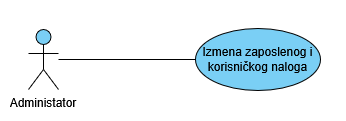
\includegraphics[width=\textwidth]{./dijagrami/dijagrami_slucajeva_upotrebe/slucaj_upotrebe_izmena_zaposlenog.png} 
	\caption{Dijagram slučaja upotrebe ,,Izmena zaposlenog i korisničkog naloga''}
\end{figure}

\begin{figure}[H]
	\centering
	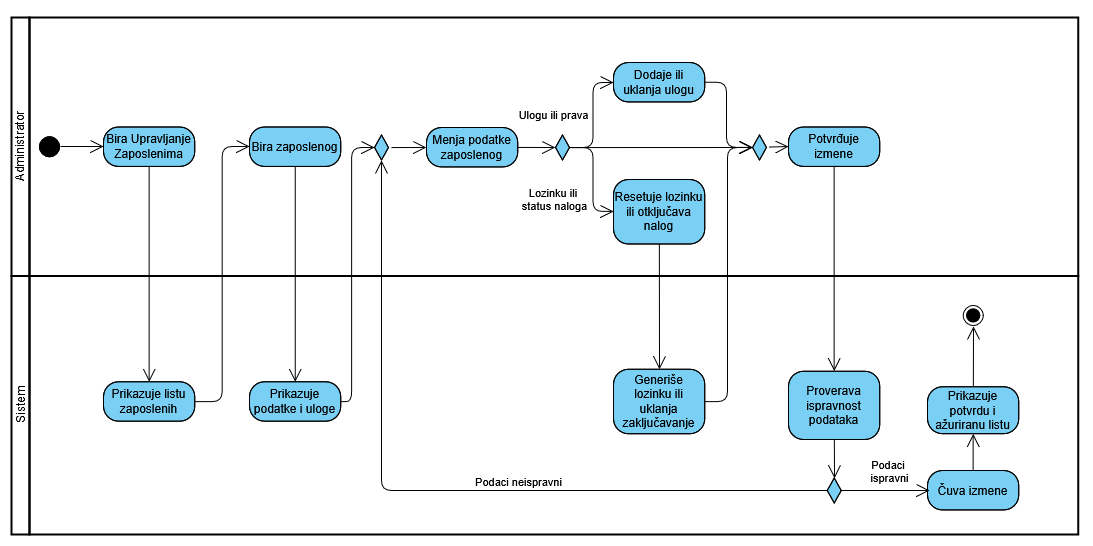
\includegraphics[width=\textwidth]{./dijagrami/dijagrami_aktivnosti/izmena_zaposlenog.png} 
	\caption{Dijagram aktivnosti ,,Izmena zaposlenog i korisničkog naloga''}
\end{figure}

\newpage